%!TEX root = ../tudkom_students__201804_v1.4.tex
\chapter{Implementierung}
\label{ch:implementation}
% This chapter should describe the details of the implementation addressing the following questions:
% 1. What are the design decisions made?
% 2. What is the environment the approach is developed in?
% 3. How are components mapped to classes of the source code?
% 4. How do the components interact with each other?
% 5. What are limitations of the implementation?
% 5 pages
Die Implementierung setzt sich zusammen aus dem Programm auf dem Wearable, der Hardware des Wearables und der Android App. Im Folgendem werden die Teilaufgaben einzeln näher betrachtet.

\section{Wearable Programm}
\subsection{Entwicklungsumgebung}
Die nRF52832 MCU wird neben dem offiziellen SDK auch von der plattformübergreifenden Softwareumgebung mBed unterstützt.
Eine plattformübergreifende Softwareumgebung zu nutzen kann es vereinfachen, den Code von der MCU auf ein anderes MCU-Modell zu portieren.
Während die Einrichtung von Mbed sehr einfach ist, da der Code im Browser geschrieben wird, unterstützt Mbed bisher leider nicht BT Mesh, weswegen es sich nicht zur weiteren Evaluation eignet \cite{site_mbedMesh}.\\
Die Arbeit nutzt das nRF5 SDK v15.3.0.
Damit das SDK vom Compiler bei Nutzung der IDE Segger Embedded Studio gefunden werden kann, muss es nach \texttt{C:\textbackslash{}nrf52\textbackslash{}sdk} entpackt werden oder die Pfade in den \texttt{.emProject}-Dateien ersetzt werden.
Hier würde es sich eignen, zukünftig eine Lösung mit systemweiten Pfadvariablen zu finden.
Bevor eine nRF52832 MCU genutzt werden kann, muss zunächst der BLE-Stack installiert werden, indem die \texttt{.hex}-Datei aus dem Softdevice 132 v6.1.1 auf die MCU übertragen wird.\\\\
Statt die IDE Segger Embedded Studio zu nutzen, kann alternativ der GCC Compiler mit einer beliebigen IDE eingesetzt werden.
Bei der komplizierten Einrichtung von GCC und den benötigten Tools ist dann zu beachten, dass bei der zum Zeitpunkt der Arbeit aktuellen Version 8-2018-q4-major der GNU Arm Embedded Toolchain\footnote{\url{https://developer.arm.com/tools-and-software/open-source-software/developer-tools/gnu-toolchain/gnu-rm}, abgerufen am 13.07.2019} ein Out-of-Range-Fehler in einer Intel-Hex-File geworfen wird.
Der Fehler kann behoben werden, indem die Datei \texttt{bin\textbackslash{}arm-none-eabi-objcopy.exe} mit der aus Version 7-2018-q2-update ersetzt wird.
Der Log kann über den Configuration Wizard in \texttt{sdk\_config.h} auf das UART-Protokoll umgestellt werden und lässt sich über das externe Programm Putty\footnote{\url{https://www.putty.org/}, abgerufen am 11.07.2019} auslesen.\\
In der Arbeit wurde wegen der einsteigerfreundlicheren Einrichtung mit der IDE Segger Embedded Studio gearbeitet.
Die IDE stürzt in der genutzten Version 4.12 leider regelmäßig ab.
Wird die IDE dagegen aktualisiert, gibt das eingebaute Debug Terminal nur noch unsichtbare Zeichen aus (vgl. \cite{site_sesDebug}).
Im Debug Terminal wird der Log, der vom RTT-Protokoll übertragen wird, angezeigt.
Wenn der Log über RTT zu schnell ist, werden Zeilen verworfen.
Um dem entgegenzuwirken, kann über Configuration Wizard in \texttt{sdk\_config.h} das \texttt{NRF\_LOG\_DEFERRED} ausgestellt werden.

\subsection{Programmaufbau}
Das Programm \texttt{main.c} ist der Einstiegspunkt der MCU.
Hier werden die vordefinierten und eigenen Module initialisiert und die Hauptschleife verwaltet.
Unter den vordefinierten Modulen sind zum Beispiel Logging, Timer und Energiemanagement.
Da das Template 700 Zeilen umfasst, wurden einige Initialisierungen in weitere Dateien ausgelagert.
Der Code \texttt{peer\_advertise.c} verwaltet die beiden Module, die zum Advertisen und zur optionalen Verbindungsverschlüsselung nötig sind.
Hier kann unter anderem eingestellt werden, wie lange das Advertisen stattfindet, bevor das Wearable automatisch in den Schlafmodus wechselt und in welchen Abständen die Pakete beim Advertisen verschickt werden.
Die Datei \texttt{board\_manager.c} steuert die LEDs und den Knopf.
Die Definition \texttt{custom\_board.h} beschreibt, wie viele LEDs und Knöpfe angeschlossen sind und an welchen Pins sie liegen.\\
Im Package \texttt{ServiceCharacteristicSensor} befindet sich der Code für die BLE-Service und den Sensor.

\subsection{BLE-Service}
Um den BLE Service und die Characteristics zu erstellen, wird nach dem Tutorial\footnote{\url{https://github.com/bjornspockeli/custom\_ble\_service\_example}, aufgerufen am 11.07.2019} eines Mitarbeiters von Nordic Semiconductor gearbeitet.
Beim Initialisieren des Services \texttt{my\_service.c} werden die beiden Characteristics \texttt{chara\_conf.c} und \texttt{chara\_data.c} erstellt und der Sensor vorbereitet.
Wenn sich ein Endgerät verbindet, startet der Sensor das Sammeln der Daten und beim Trennen wird er angehalten und zurückgesetzt.\\\\
Erfasst der Sensor einen neuen Datensatz, wird der Datensatz im Wert der Characteristic \texttt{chara\_data.c} veröffentlicht.
Da die Werte erst zum nächsten Connection Interval verschickt werden, müssen sie vom BLE-Stack zwischengespeichert werden.
Ist der Buffer allerdings voll, wird beim Einfügen ein \texttt{NRF\_ERROR\_RESOURCES}-Fehler von der Funktion \texttt{sd\_ble\_gatts\_hvx} geworfen.
Die Minimalgröße des TX-Buffers kann vor dem Initialisieren des BLE-Stacks mit der Konstanten \texttt{TX\_QUEUE\_SIZE} manuell gesetzt werden und ist standardmäßig 0.
Es ist möglich, die tatsächliche Größe abzuschätzen, da bei einer Teilentleerung des Buffers ein \texttt{TX\_COMPLETE}-Event geworfen wird.
Wird beim Einfügen in den TX-Buffer ein Counter hoch- und bei einem \texttt{TX\_COMPLETE}-Event runtergezählt, kann die Kapazität bei einem \texttt{NRF\_ERROR\_RESOURCES}-Fehler erhalten werden.
Nach diesem Verfahren wurde bei dem Programm dieser Arbeit ermittelt, dass die tatsächliche Kapazität etwa 3 Einheiten mehr als die Minimalgröße beträgt.\\
Wenn betrachtet wird, dass die verwendeten IMUs die Daten mit bis zu 1600 Hz erfassen können, ist die benötigte Buffergröße $1600 Hz * 4s = 6400$ wegen des maximalen Connection Intervals von 4 Sekunden.
Den Buffer auf diese Größe zu setzen muss aber nicht sinnvoll sein, da nicht sichergestellt ist, dass in einem Connection Interval der komplette Buffer geleert wird.
Das ist von der Übertragungsgeschwindigkeit abhängig, die sich auch aus der Empfangsqualität und der Paketverlustrate ergibt.
Ist der Buffer größer als die Übertragungsgeschwindigkeit erlaubt, wird der Buffer volllaufen, Sensordaten werden letztendlich verworfen und die eingereihten Sensordaten kommen erst in einem späteren Connection Interval an, sodass eine Verzögerung entsteht.
Wird der Buffer kleiner gewählt, passen nicht alle Sensordaten hinein und müssen verworfen werden.\\\\
Im Optimalfall sollte die Übertragungsgeschwindigkeit maximiert werden und der Buffer dazu passend mit etwas Spielraum nach unten gewählt werden.
Die maximale MTU-Größe kann mit dem Configuration Wizard in \texttt{sdk\_config.h} mit der Konstanten \texttt{NRF\_SDH\_BLE\_GATT\_MAX\_MTU\_SIZE} geändert werden.
Sowohl eine größere MTU-Größe als auch ein größerer TX-Buffer benötigt zusätzlichen Platz in der BLE-Stack-Section vom RAM.
Der reservierte Platz im RAM kann eingestellt werden mit der Konstanten \texttt{RAM\_START} unter den \texttt{linker\_section\_placement\_macros} in der SES-Projekt-Datei, zu finden mit der Endung \texttt{.emProject}.
Wird zu wenig Platz reserviert, startet das Programm nicht.\\\\
Der Wert, der hinter der Characteristic \texttt{chara\_data.c} steht, besteht aus den Komponenten in Abbildung \ref{lst:imuData}.
Aus dem Inhalt ergibt sich eine Größe von 16 Byte.
Das MSb des Zeitstempels wird nicht genutzt, da auf Endgeräten genutzte Hochsprachen oft keine vorzeichenlosen Werte interpretieren können.
Die LSM6DSL IMU speichert den Zeitstempel im 6.4 ms Format.
Es ist sinnvoll, dieses Zeitformat auf das schnellste Datenerfassungsintervall von $\frac{1s}{1600Hz} = 0.625 ms$ zu normalisieren, sodass beide Sensoren dieselbe Zeiteinheit liefern können.
Allerdings ist die Zeiteinheit der LSM6DSL IMU kein Vielfaches, sodass Rundungsfehler entstehen würden.
Beim BMI160 wird die Einheit der Zeitstempel mit 0.625 ms übertragen.
Hier wird der Zeitstempel aber von der MCU berechnet, sodass er nicht mehr korrekt wäre, wenn die FIFO der IMU überläuft.
Deswegen wird die FIFO des BMI160 nur zu 75 \% gefüllt.\\
Der LSM6DSL arbeitet zudem mit leicht verschiedenen Frequenzen als der BMI160.
Die Unterschiede können in Tabelle \ref{tab:imuFreq} betrachtet werden. \cite {datasheet_lsm6dsl} \cite{datasheet_bmi160}\\
\begin{minipage}{\linewidth}
	\centering
	\captionof{table}{IMU Frequenzen (in Hz)}
	\label{tab:imuFreq}
	\begin{tabular}{l|l|l|l|l|l|l|l}
		BMI160 & 25 & 50 & 100 & 200 & 400 & 800 & 1600\\
		LSM6DSL & 26 & 52 & 104 & 208 & 416 & 833 & 1666\\
  \end{tabular}
\end{minipage}\\\\
In Zukunft sollte eine einheitliche Lösung gefunden werden.
Zur Berechnung der Statistiken soll vorerst mit unverarbeiteten Daten gearbeitet werden und am Smartphone umgerechnet werden.
\begin{figure}[hbtp]
	\lstinputlisting{res/imuData.c}
	\caption{Inhalt von Characteristic \texttt{chara\_data.c}}
	\label{lst:imuData}
\end{figure}\\
Schickt das Endgerät dem Wearable mit der Characteristic \texttt{chara\_conf.c} eine neue Konfiguration, wird versucht, die Konfiguration anzuwenden.
Ändert sich die Konfiguration, wird sie dem Endgerät mit einem Notify mitgeteilt.

\subsection{IMU Integration}
% durch pattern sensoren einfach austauschbar
Damit die IMU, aber auch die verwendeten Protokolle, leicht austauschbar sind, wurde der Code für die IMU aufgeteilt.
Die Definitionen in \texttt{imu.h} soll dabei jede IMU implementieren und ist die Schnittstelle zum BLE-Service.
Der Header \texttt{*\_protocol.h} deklariert das Protokoll, mit dem die IMU mit MCU kommuniziert, das heißt SPI oder I2C.
Mit der Konstanten \texttt{PROTOCOL\_SPEED} lässt sich die Geschwindigkeit des Protokolls ändern.
Der Header \texttt{*\_get\_data.h} deklariert die Art, wie Daten gesammelt werden.
Die Implementierungen können unterschiedliche Interrupts nutzen wie FIFO-Full oder Data-Ready.
Um die Implementierung auszutauschen muss eine andere \texttt{.c}-Datei gelinkt werden, indem die entsprechende Zeile im \texttt{.emProject}-Projekt geändert wird.\\
Die IMU soll mithilfe der Callback-Funktion \texttt{bool (*send\_data)(imu\_data\_t)} die gemessenen Werte an die MCU zurück liefern.\\\\
Beim Testen mit dem Prototypen ist das Problem, das in Abbildung \ref{fig:daten_vorher} veranschaulicht wird, aufgekommen.
\begin{figure}[!hbtp]
	\centering
	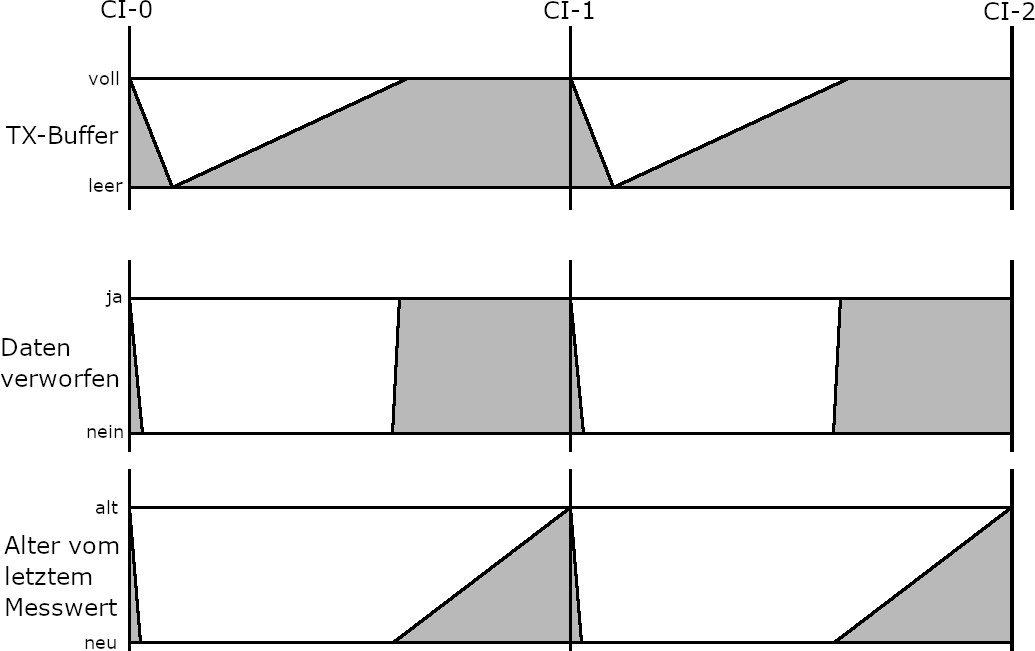
\includegraphics[width=0.76\linewidth]{res/datenVorher.jpg}
	\caption{Darstellung des Datenstaus. CI = Connection Interval}
	\label{fig:daten_vorher}
\end{figure}
Wenn die Sensordatenrate zu schnell für den TX-Buffer oder dem Connection Interval ist, empfängt das Endgerät die Sensordaten mit wechselnder Verzögerung.
Wurde der TX-Buffer gerade durch ein Connection Interval geleert, werden alle nächsten Sensordaten in den Buffer eingetragen, bis der Buffer voll ist.
Danach werden alle Sensordaten bis zum nächsten Connection Interval verworfen.\\
Prinzipiell kann das Problem gelöst werden, indem der Connection Interval verkleinert, der TX-Buffer vergrößert oder die Datenmenge verkleinert wird.
Da die Größe vom TX-Buffer nach der Initialisierung nicht geändert werden kann und von der veränderlichen Durchsatzrate beschränkt ist, reicht es nicht unbedingt alleine aus, diesen Parameter zu variieren.
Der Connection Interval wird vom Endgerät bestimmt.
Das Wearable kann eine neue Geschwindigkeit vorschlagen.
Können sich Wearable und Endgerät nicht einigen, wird die Verbindung getrennt.
Das würde das Nutzungserlebnis stark negativ beeinflussen.
Um die Datenmenge zu reduzieren, kann der Sensor langsamer gestellt oder absichtlich Daten verworfen werden.
Während das Zweite eine feinere Einstellung ermöglicht, ist das Erste stromsparender.\\
Deswegen wird ein Algorithmus eingesetzt, der die Geschwindigkeit vom Sensor herabsetzt, wenn ein neues Connection Interval vorliegt oder der Nutzer eine neue Geschwindigkeit setzen möchte.
Das Ergebnis soll dem in Abbildung \ref{fig:daten_nachher} veranschaulichte Verhalten nachkommen.
\begin{figure}[!hbtp]
	\centering
	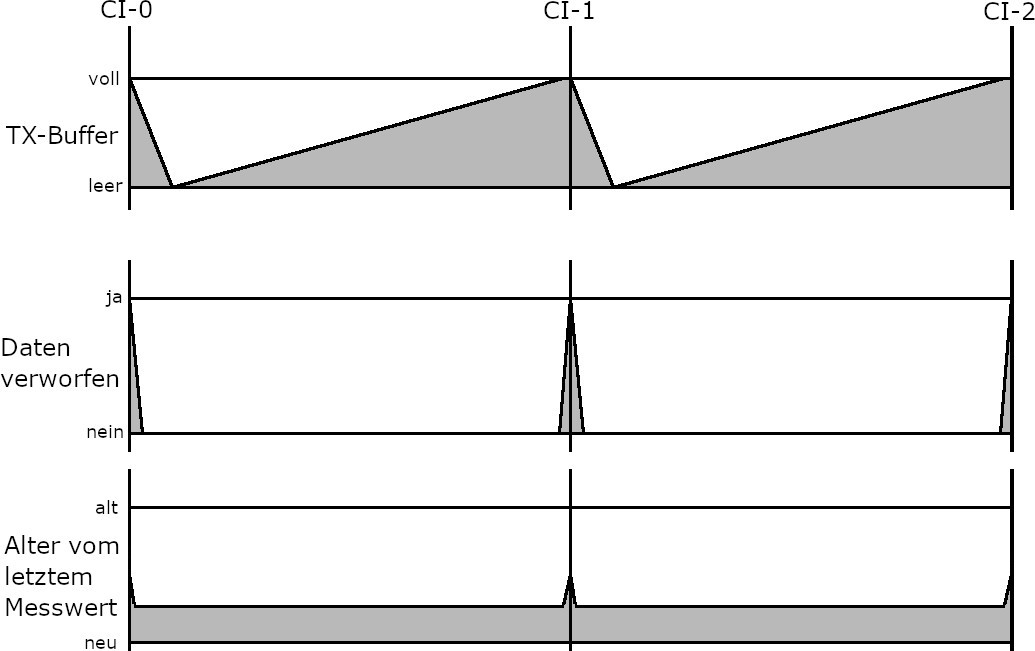
\includegraphics[width=0.76\linewidth]{res/datenNachher.jpg}
	\caption{Lösung des Datenstaus}
	\label{fig:daten_nachher}
\end{figure}
Der Rückgabewert der Callback-Funktion \texttt{bool (*send\_data)(imu\_data\_t)} gibt an, ob die Daten in den TX-Buffer eingefügt werden konnten oder der Buffer schon voll ist.
Der Parameter \texttt{uint16\_t buffer\_size} der Funktion \texttt{imu\_init} entspricht der eingestellten Größe des TX-Buffers.
Die Funktion \texttt{void imu\_on\_new\_interval(\allowbreak{}uint16\_t buffer\_clear\_interval)} wird aufgerufen, wenn die Geschwindigkeit der BLE-Verbindung sich geändert hat.
Der Parameter \texttt{buffer\_clear\_interval} ist dabei das Connection Interval.
Die Geschwindigkeit wird gespeichert und in den weiteren Aufrufen von der Funktion \texttt{void imu\_speed\_set(\allowbreak{}imu\_speed\_t speed)} verwendet.\\
Der Algorithmus wird am Beispiel der LSM6DSL IMU mit FIFO-Threshold Interrupt beschrieben (\texttt{lsm\_get\_data\_fifo.c}).
Zunächst werden in Abbildung \ref{lst:algoPre} die Konstanten für den Sensor berechnet.
\begin{figure}[t]
	\lstinputlisting{res/algoPre.c}
	\caption{Vorbereitung des Algorithmus}
	\label{lst:algoPre}
\end{figure}
Die Geschwindigkeit wird in Abbildung \ref{lst:algo} berechnet.
\begin{figure}[bhtp]
	\lstinputlisting{res/algo.c}
	\caption{Berechnung der Geschwindigkeit}
	\label{lst:algo}
\end{figure}
Dabei wird mit jeder Iteration berechnet, ob der Sensor in einem Connection Interval mehr Daten erfasst, als in den Buffer passen.
Falls es zu viele sind, wird die Geschwindigkeit herunter gesetzt, wenn sie nicht auf dem kleinsten möglichen Wert ist.
Zum Schluss wird die Geschwindigkeit wieder um einen Schritt erhöht.
Da ein Schritt eine Halbierung oder Verdopplung der Datenrate bedeutet und damit die Lösung nicht den perfekten Punkt für die Datenrate treffen kann, wird dem Programm des Endgeräts freigestellt, ob es die Datenrate nochmals halbieren wird.
Durch die Variable \texttt{bool didGoLowerOnceAndNowOk} wird sichergestellt, dass die Datenrate nicht höher als vom Endgerät eingestellt wird und, dass der Algorithmus am Ende nicht von der langsamsten Geschwindigkeit erhöht, falls die langsamste Einstellung immer noch zu schnell ist.
Falls die Sensordatenrate sehr langsam im Vergleich zum Connection Interval ist, soll nicht gewartet werden, bis die FIFO mit 227 Paketen voll ist.
Dann würden in einigen Connection Intervals gar keine und anschließend 227 Pakete in Einem geschickt werden.
Deswegen wird der FIFO-Threshold wie in Abbildung \ref{lst:algoPost} eingestellt.
Damit soll die FIFO mindestens ein Mal pro Connection Interval ausgelesen werden.
\begin{figure}[hbtp]
	\lstinputlisting{res/algoPost.c}
	\caption{Berechnung des Thresholds}
	\label{lst:algoPost}
\end{figure}\\
Bei der Implementierung des Algorithmus mussten weitere Probleme gelöst werden.\\\\
Der Treiber der LSM6DSL IMU stellt die Funktion \texttt{lsm6dsl\_fifo\_raw\_data\_get} zum Auslesen der FIFO bereit.
Da die FIFO eine Größe von 4096 Byte hat, lässt sie sich mit der Funktion wegen dem Parameter \texttt{uint8\_t len} nicht komplett auslesen.
Das ergibt wenig Sinn und auch das Datenblatt begründet die Einschränkung nicht.
Schaut man in die Implementierung in Abbildung \ref{lst:fifoRead}, stellt man fest, dass sie nur eine weitere Funktion aufruft.
Der vierte Parameter der Funktion \texttt{lsm6dsl\_read\_reg} ist vom Typ \texttt{uint16\_t}.
Somit lässt sich die allgemeinere Funktion stattdessen nutzen, um die komplette FIFO auszulesen.
Es ist davon auszugehen, dass es sich um einen Fehler im Treiber handelt.
\begin{figure}[hbtp]
	\lstinputlisting{res/fifoRead.c}
	\caption{Auslesen der FIFO}
	\label{lst:fifoRead}
\end{figure}\\
Unabhängig vom vorherigen Problem, gibt es ein Ähnliches bei der Nutzung von EasyDMA (siehe Abschnitt \ref{ch:mcu}).
Für eine einfache Transaktion von SPI oder I2C ist der Buffer durch die Größe vom 8 Bit Register \texttt{MAXCNT} begrenzt (siehe Abschnitt 10, 31 und 33 in \cite{datasheet_nrf52832}).
Da ein Byte für die Adresse reserviert ist, können 254 Datenpakete pro Transaktion verschickt werden.
Diese Einschränkung wurde in Abbildung \ref{lst:algoPre} in Zeile 9ff und Abbildung \ref{lst:algoPost} in Zeile 7f beachtet.
Beim Auslesen der FIFO werden dafür mehrere Transaktionen durchgeführt, bis die FIFO leer ist.
Alternativ hätte man die List-Funktion der EasyDMA oder die nRF52840 MCU, die 16 Bit für den Buffer bereitstellt \cite{datasheet_nrf52840}, nutzen können.

\section{Wearable Hardwareumsetzung}
Zur Entwicklung der Software und des Hardwareprototypen wurde das nRF52 DK mit der IMU auf den Evaluationsplatinen mit Jumperkabeln verbunden.
Zur Evaluation sollen die Platinen durch kleinere Alternativen ersetzt werden.
Da kurzzeitig ein Reflowofen verfügbar war, konnten selbst kleinste QFN-Bauteile verlötet werden.
Die LSM6DSL IMU wurde als QFN-Chip und die MCU in Form der Laird BL651 verbaut.
Die Platine von Laird bietet den Vorteil gegenüber der MCU als Chip, dass kein Vorwissen über Antennen nötig ist.
Dieser Abschnitt entnimmt seine Informationen den Datenblättern der Bauteile.\\
An die MCU kann optional ein 32.768 kHz Taktgeber angeschlossen werden.
Ohne den Taktgeber wird das Taktsignal von anderen Taktgebern synthetisiert.
Der Taktgeber muss innerhalb der von der MCU vorgegebenen Spezifikation liegen und benötigt zwei Kondensatoren zum Schwingen.
Die Kapazität der Kondensatoren $C$ lässt sich mit den Formeln und Werten \ref{eq:quatz1} bis \ref{eq:quatz2} auf 6 pF bestimmen. \cite{datasheet_nrf52832}
\begin{gather}
  \label{eq:quatz1}
	CL = \cfrac{C'^2}{2*C'}\\
	C' = C + C_{pcb} + C_{pin}\\
\intertext{mit den Werten}
	CL = 7 pF\text{: Lastkapazität des ausgewählten Taktgebers}\\
	C_{pcb} \simeq 4 pF\text{: Kapazitäten durch die Leiterbahnen und Platine}\\
  \label{eq:quatz2}
	C_{pin} = 4 pF\text{: Kapazität des Pins der MCU}
\end{gather}\\
Die Pins P0.22 bis P0.31 der MCU dürfen nicht hochfrequent betrieben werden, da es die BLE-Kommunikation negativ beeinflussen kann \cite{datasheet_nrf52832}.
Im Design der Platine wurde deswegen auf diese Pins verzichtet.
Der Interrupt2 Pin der IMU konnte dadurch leider platzbedingt nicht verbunden werden.
In zukünftigen Versionen der Platine sollte er wenn möglich angeschlossen werden, um der Softwareentwicklung mehr Möglichkeiten offen zu lassen.\\
An den zwei Spannungspins der IMU und dem Spannungspins der MCU sind 100 $\mu$F Kondensatoren angebracht.
Sie dienen zur Abkopplung der Komponenten bei Lastschwankungen und sind auch in den Referenzimplementierungen vorhanden \cite{datasheet_nrf52832} \cite{datasheet_lsm6dsl}.
Die ausgewählten LEDs haben eine Vorwärtsspannung von 1.8 V und einen Nennstrom von 2 mA.
Um diese Vorgaben bei einem Batterielevel von 2 V bis 3 V einzuhalten, sind jeweils 191 Ohm Widerstände vorgeschaltet.
Als Farben der LEDs wurden rot und gelb gewählt, da die Farben eine hohe Wellenlänge haben und dadurch energieärmer sind.
Wird die rote LED der Gelben in der Nutzung präferiert, steigert sich aus dem selben Grund die Effizienz des Wearables minimal.
Zur Programmierung des Chips wurde ein Cortex-M-Debug\footnote{\url{http://infocenter.arm.com/help/topic/com.arm.doc.faqs/attached/13634/cortex_debug_connectors.pdf}, aufgerufen am 18.07.2019} Anschluss angebracht.
Damit lässt er sich vom nRF52 DK mit dem passenden Kabel programmieren.
Um die Stromaufnahme zu evaluieren, ist die Spannungsversorgung der Platine über zwei Pins, die 2.54 mm voneinander entfernt sind, offen zugänglich.
Soweit verfügbar wurden alle Komponenten in der Größe 0603 gewählt, damit sie mit einem Lötkolben eingelötet oder ausgetauscht werden können.
Eine vollständige Liste der Komponenten ist in Tabelle \ref{tab:bom} zu finden.\\

\begin{minipage}{\linewidth}
	\captionof{table}{Bill of Materials (BOM)}
	\label{tab:bom}
	\begin{tabularx}{\linewidth}{l|X|l|>{\hsize=.3\hsize}X}
		Komponente & Typ & Anzahl & Name im Schaltplan\\
		\hline
		Laird BL652-SA-01 & nRF52832 MCU & 1 & IC1\\
		STMicroelectronics LSM6DSL & LSM6DSL IMU & 1 & U1\\
		ECS Inc ECS-.327-7-34R & 32.768 kHz Taktgeber mit 7 pF Ladekapazität und 50 kOhm ESR & 1 & Y1\\
		Yageo CC0603CRNPO9BN6R0 & 6 pF Kondensator für Taktgeber & 2 & C2, C3\\
		Yageo CC0603JRX7R9BB104 & 0.1 $\mu$F Kondensator zur Abkopplung & 3 & C1, C4, C5\\
		Vishay TLMY1000-GS08 & Gelbe LED & 1 & LED1\\
		Vishay TLMS1000-GS08 & Rote LED & 1 & LED2\\
		Vishay CRCW0603191RFKEA & 191 Ohm Widerstand für LEDs & 2 & R1, R2\\
		Keystone Electronics 3008 & CR2450 Knopfzellenhalter & 1 & CR2450\\
		Panasonic EVQ-Q2B03W & Taster & 1 & S1\\
		CNC-Tech 3220-10-0300-00 & Cortex-M-Debug Buchse & 1 & J2\\
  \end{tabularx}
\end{minipage}\\\\
Bei der Erstellung des Schaltplans, in Abbildung \ref{fig:schematic} zu sehen, musste bereits beachtet werden, wo sich die Pins physisch an den Komponenten befinden, damit sich die Verbindungen nicht überschneiden.
Die Komponenten lassen sich mit der letzten Spalte von Tabelle \ref{tab:bom} zuordnen.
Die Komponente VCC.GND beinhaltet die besagten Pins zur externen Spannungsversorgung.
\begin{figure}[p]
	\centering
	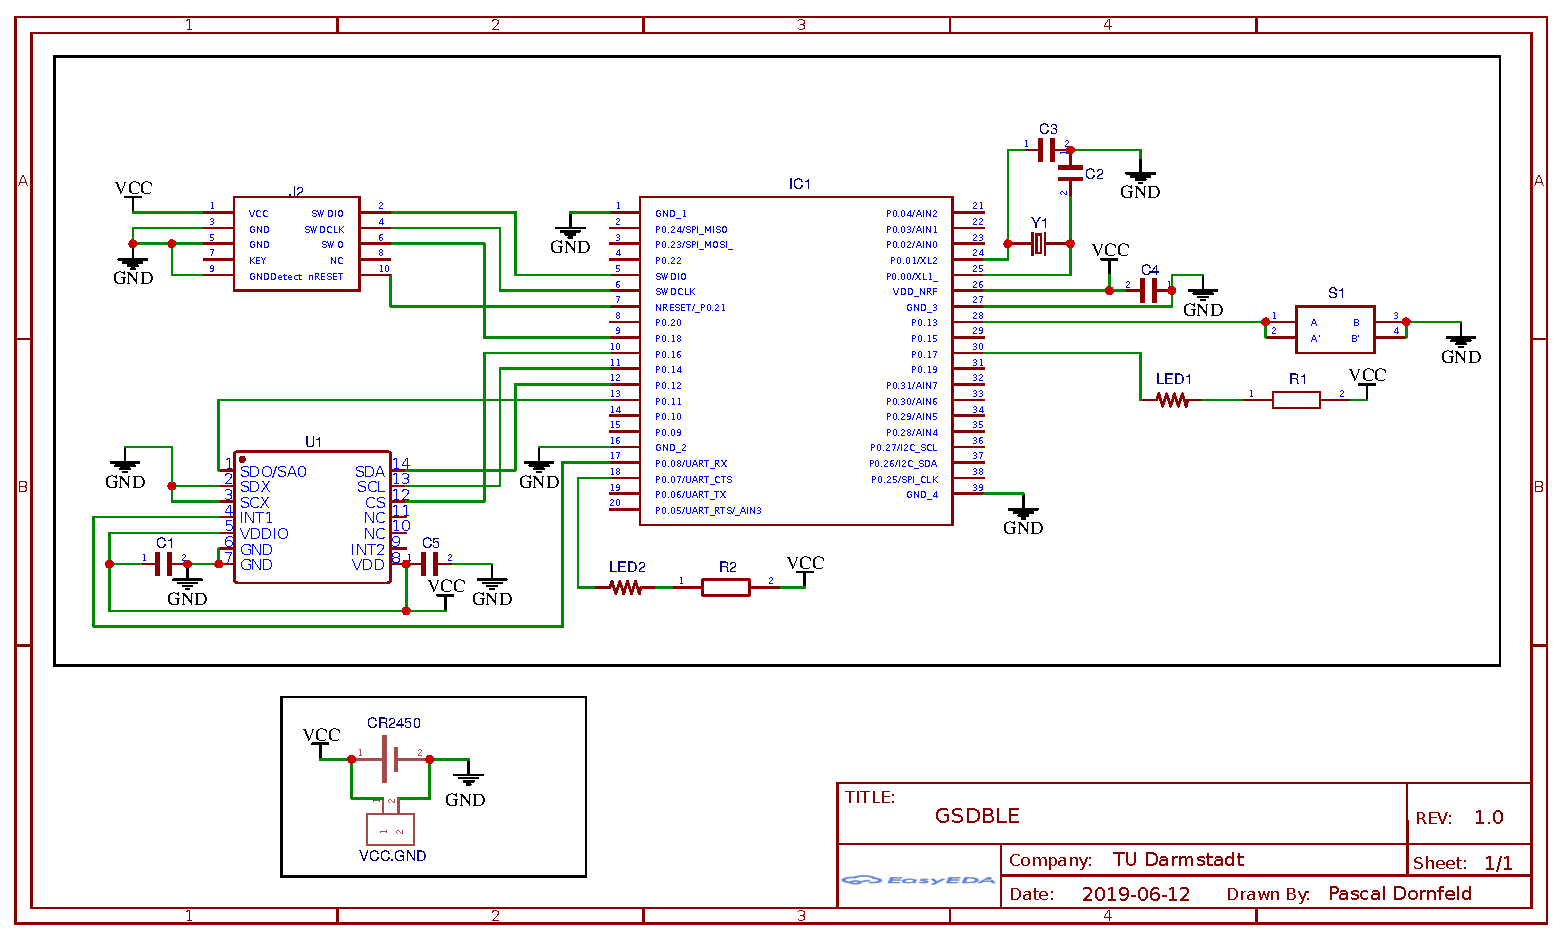
\includegraphics[height=0.8\linewidth,angle=90]{res/schematic.pdf}
	\caption{Schaltplan der Platine}
	\label{fig:schematic}
\end{figure}\\
Die Platine wurde nach dem Entwurf in Abbildung \ref{fig:platinenlayout} bei JLCPCB\footnote{\url{https://jlcpcb.com/}, aufgerufen am 18.07.2019} angefertigt.
Die roten und blauen Stellen sind Kupferverbindungen.
Die größeren Felder sind die Masseflächen.
Die grauen Vias verbinden die Unterseite mit der Oberseite.
Während sich auf der Unterseite nur die Batterie befindet, sind die restlichen Komponenten auf der Oberseite.
Das freie Rechteck in der linken unteren Ecke enthält kein Metall, da sich hier die Antenne befindet und sonst negativ beeinflusst werden würde.
An der Rückseite erkennt man, dass die Größe der Platine durch die Batterie und der Antenne vorgegeben sind.
Die Verbindungen zur Spannungsversorgung sind dicker ausgeführt, damit sie weniger Widerstand bieten.
Normalerweise wird die Unterseite der Platine genutzt, wenn Verbindungen sich überschneiden.
Die Unterseite ist fast komplett durch die Batterie belegt.
Über den Kupferleitungen ist eine isolierende Lackschicht, die vor Kurzschlüssen durch die Batterie schützen würde.
Da die Knopfzelle allerdings beim Einlegen und Entfernen über die Oberfläche reibt, ist zu erwarten, dass die Lackschicht sich abträgt und dann nicht mehr schützt.
Deswegen mussten Überschneidungen komplett vermieden werden.
\begin{figure}[hbtp]
	\centering
	\subfloat[Vorderseite]{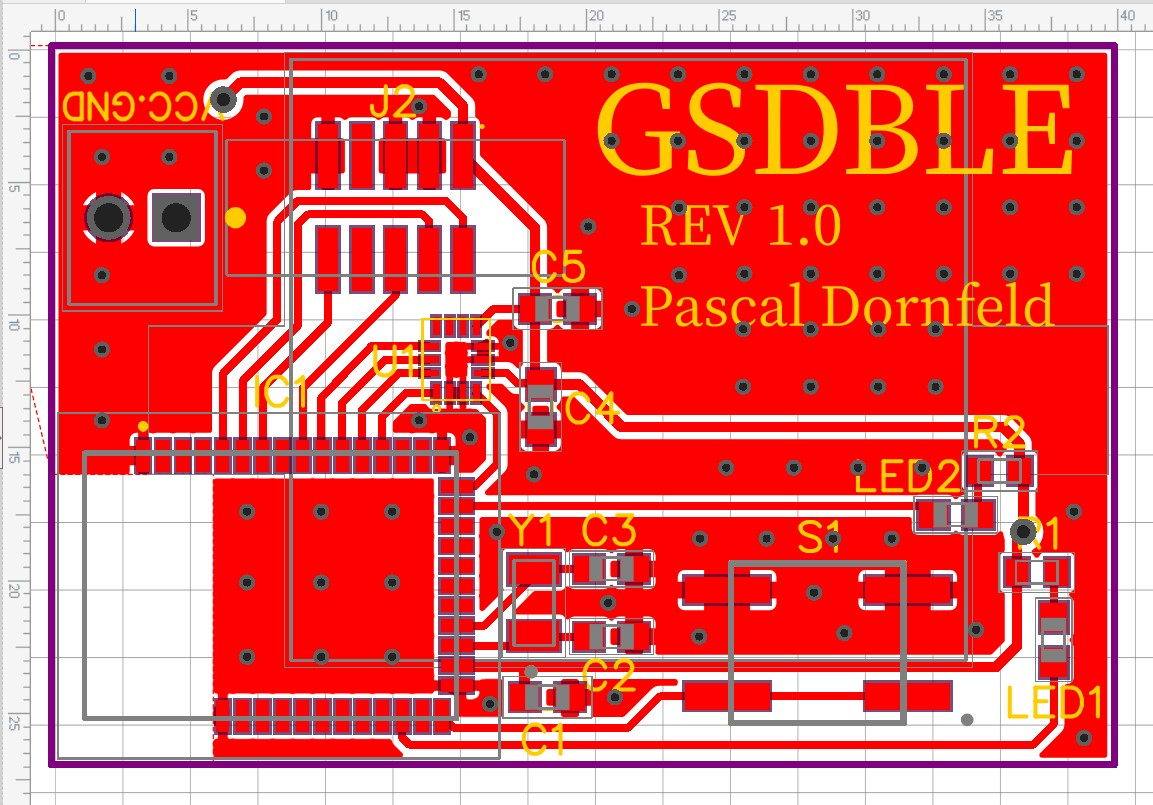
\includegraphics[width=0.5\linewidth]{res/platineFront.jpg}}
	\subfloat[Rückseite]{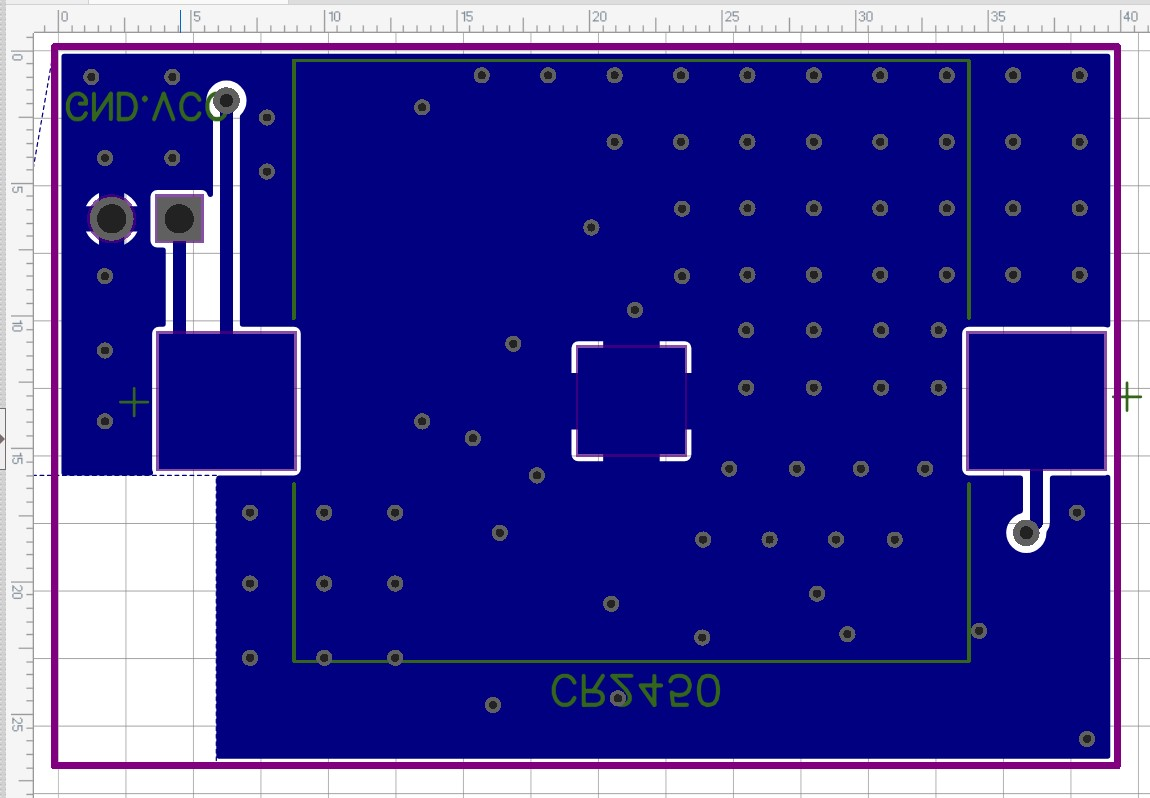
\includegraphics[width=0.5\linewidth]{res/platineBack.jpg}}
	\caption{Platinenlayout}
	\label{fig:platinenlayout}
\end{figure}\\
Die fertige Platine ist in Abbildung \ref{fig:platine} zu finden.
Zum Größenvergleich sind CR2032 und CR2450 Knopfzellen und das nRF52 DK mit abgebildet.
\begin{figure}[hbtp]
	\centering
	\includegraphics[width=0.5\linewidth]{res/gsdble.jpg}
	\caption{Fertig bestückte Platine im Größenvergleich}
	\label{fig:platine}
\end{figure}\\

\section{Android App}
Die App wurde mit dem Android SDK geschrieben, das speziell für Android Smartphones entwickelt wurde.
Obwohl Java weiter verbreitet und auch vom SDK unterstützt wird, ist die App in der Sprache Kotlin geschrieben, da sie sinnvolle Erweiterungen zu Java bietet wie Datenklassen und funktionelle Programmierung und der Code gleichzeitig mit Javacode substituierbar ist.\\
Die App wurde für Android 9.0 kompiliert und getestet und ist bis Android 5.0 abwärtskompatibel.
Ältere Versionen werden nicht unterstützt, da die Methode \texttt{no.\allowbreak{}nordicsemi.\allowbreak{}android.\allowbreak{}ble.\allowbreak{}BleManager\#\allowbreak{}requestConnectionPriority} Android 5.0 erfordert und gebraucht wird, um den Connection Interval des BLE-Stacks zu setzen.\\
Beim Start der App wird die \texttt{ConnectActivity} gestartet.
Sie enthält nur einen Knopf.
Drückt der Nutzer auf den Knopf, sucht das Smartphone nach Geräten, die mit dem Namen 'GSDBLE' advertisen.
Der Knopf ist ausgegraut, wenn das Smartphone kein BLE unterstützt oder der Nutzer der App keine Rechte für die Nutzung von Bluetooth gegeben hat.
Wenn ein Wearable gefunden wurde, wechselt die App auf die \texttt{ConnectionOverviewActivity}.
Dabei wird das gefundene Wearable im Intent \texttt{EXTRA\_DEVICE} übergeben.\\
Die Activity \texttt{ConnectionOverviewActivity} verbindet sich mit dem Wearable, sucht nach den Services und Characteristics und setzt das Notify-Bit bei den Characteristics.
Das Android SDK bietet Klassen zur Verbindung mit BLE.
Hier hat sich herausgestellt, dass alle Befehle asynchron laufen.
Dabei ist problematisch, dass die Befehle nicht in einer Schlange verwaltet werden, sondern ein Befehl ignoriert wird, wenn der Vorherige noch nicht abgeschlossen ist.
Deswegen wurde auf die Bibliothek von Nordic\footnote{\url{https://github.com/NordicSemiconductor/Android-BLE-Library}, aufgerufen am 18.07.2019} zugegriffen, die die Klassen des SDK besser zugänglich macht.\\
Die Klasse \texttt{Manager} verwaltet die Verbindung.
Die Activity \texttt{ConnectionOverviewActivity} dagegen verwaltet die graphische Oberfläche.
In der Activity werden verschiedene Statistiken graphisch angezeigt.
Darunter sind die Sensordaten, aber auch z.B. die empfangenen Daten pro Sekunde.
Über Slider lassen sich Parameter einstellen.
Die Parameter sind die MTU, das Connection Interval und die Sensordatenrate.
Da die IMUs verschiedene Zeiteinheiten und unterschiedliche Datenraten besitzen, lässt sich der Sensor mit einem Slider einstellen, damit die Statistiken korrekt berechnet werden.
Das Connection Interval lässt sich in den Schritten Low, Balance und High ändern.
Das entspricht den Werten 100 - 125 ms, 30 - 50 ms und 11.25 - 15 ms.
Diese Vorgabe besteht durch die Konstanten der Klasse \texttt{android.bluetooth.BluetoothGatt} im Android SDK.
Jedes Teil ist davon ein eigenes Fragment aus den Dateien \texttt{ConfigFragment} oder \texttt{Graphfragment}.
Die abstrakte Klasse \texttt{Graphfragment} empfängt Daten und fügt sie in die Liste \texttt{internalData} ein.
Wenn die Liste zu voll ist, werden die ältesten Daten entfernt.
Die Daten sollen dann von der Graphenbibliothek angezeigt werden.
Da sie in einem anderen Thread arbeitet und es sonst zu Race Conditions kommt, wird von der Liste \texttt{internalData} ein Snapshot in \texttt{data} für die Graphenbibliothek erstellt.\\
Die Werte der Characteristics sind in den Modelklassen \texttt{ImuConfig} und \texttt{ImuData} realisiert.
Sie bieten die Möglichkeit die Werte in ein \texttt{ByteArray} umzuwandeln und wieder zurück.

\section{Zusammenfassung}
Die Einrichtung der Entwicklungsumgebung der MCU ist leider kompliziert und bedarf vieler Umwege.
Die Installation von Android Studio dagegen läuft problemlos.
Von den Entwickler der MCU und Drittanbietern sollte hier nachgebessert werden.\\
Um den Datenstau zu umgehen, der durch die drei Buffer in MCU und IMU entsteht, berechnet ein Algorithmus die Parameter zur korrekten Umfüllung.
Der Hardwareentwurf ist erfolgreich verlaufen, sodass ein Wearable zur Evaluation bereit steht.
In der Android App werden dafür Daten gesammelt, die statistisch ausgewertet werden können.
